\begin{figure}[h]
  \centering
  \begin{subfigure}[b]{0.45\textwidth}
    \centering
    
\begin{tikzpicture}
            % Body
      \fill[gray!50] (0,0) circle (1);
      
      % Ears
      \fill[gray!50] (-0.7,0.7) -- (0,1.3) -- (0.7,0.7) -- cycle;
      \fill[gray!50] (-0.7,0.7) arc (180:360:0.7cm and 0.2cm);
      
      % Face
      \fill[white] (0,0) circle (0.8);
      
      % Eyes
      \fill[black] (-0.3,0.3) circle (0.1);
      \fill[black] (0.3,0.3) circle (0.1);
      
      % Nose
      \fill[black] (0,0) circle (0.05);
      
      % Whiskers
      \draw[black, thick] (-0.4,0) -- (-1.5,0);
      \draw[black, thick] (0.4,0) -- (1.5,0);
      \draw[black, thick] (-0.4,-0.2) -- (-1.5,-1);
      \draw[black, thick] (0.4,-0.2) -- (1.5,-1);
      \draw[black, thick] (-0.4,0.2) -- (-1.5,1);
      \draw[black, thick] (0.4,0.2) -- (1.5,1);
      
      % Whiskers reflection
      \draw[white, thick] (-0.4,-0.05) -- (-1.5,0.7);
      \draw[white, thick] (0.4,-0.05) -- (1.5,0.7);
      \draw[white, thick] (-0.4,0.15) -- (-1.5,-0.7);
      \draw[white, thick] (0.4,0.15) -- (1.5,-0.7);
      
      % Mouth
      \draw[black, thick] (-0.3,-0.4) .. controls (0,-0.8) .. (0.3,-0.4);
      
      % Whiskers reflection
      \draw[white, thick] (-0.3,-0.35) .. controls (0,-0.75) .. (0.3,-0.35);
      
    \end{tikzpicture}
    \caption{ChatGPT 3.5 is \emph{okay} at drawing a cat using the tikz package.}
  \end{subfigure}
  \hfill
  \begin{subfigure}[b]{0.45\textwidth}
    \centering
    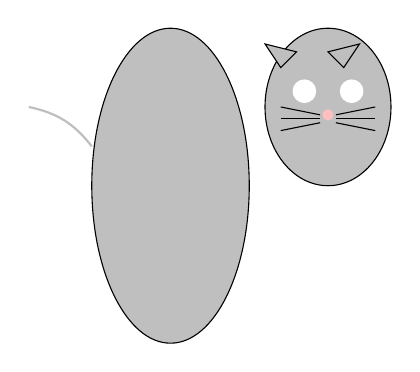
\begin{tikzpicture}
          % Draw the body
    \draw[fill=gray!50] (2,1) ellipse (1cm and 2cm);
    % Draw the head
    \draw[fill=gray!50] (4,2) ellipse (0.8cm and 1cm);
    % Draw the eyes
    \fill[white] (3.7,2.2) circle (0.15cm);
    \fill[white] (4.3,2.2) circle (0.15cm);
    % Draw the nose
    \fill[pink] (4,1.9) circle (0.07cm);
    % Draw the ears
    \draw[fill=gray!50] (3.2,2.8) -- (3.6,2.7) -- (3.4,2.5) -- cycle;
    \draw[fill=gray!50] (4.4,2.8) -- (4.0,2.7) -- (4.2,2.5) -- cycle;
    % Draw the tail
    \draw[thick, gray!50] (1.0,1.5) to [bend right=20] (0.2,2.0);
    % Draw the legs
    \draw[thick, gray!50] (2.3, 0) -- ++(0, -0.7);
    \draw[thick, gray!50] (1.7, 0) -- ++(0, -0.7);
    % Draw the whiskers
    \draw (4.1,1.8) -- ++(0.5,-0.1);
    \draw (4.1,1.85) -- ++(0.5,0);
    \draw (4.1,1.9) -- ++(0.5,0.1);
    \draw (3.9,1.8) -- ++(-0.5,-0.1);
    \draw (3.9,1.85) -- ++(-0.5,0);
    \draw (3.9,1.9) -- ++(-0.5,0.1);
    \end{tikzpicture}
    \caption{ChatGPT 4 draws a more detailed image, that is only slightly harrowing.}
  \end{subfigure}
  \caption{Note that, though neither drawing is good, both are much better than I could do.}
\end{figure}